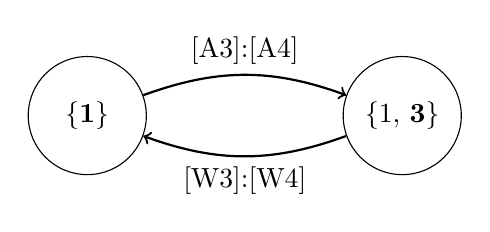
\begin{tikzpicture}[scale=0.2, state/.style={draw=black,circle,inner sep=0pt}]
		\node [state, minimum size=1.5cm] (s1) at (0,0) {\{\textbf{1}\}};
		\node [state, minimum size=1.5cm] (s2) at (20,0) {\{1, \textbf{3}\}};
	%\draw[arrow](B1.west) to [out=190,in=170] node[above]{Flow: $\alpha$ } (S1.west);
	\draw [thick, ->] (s1) to[out=20, in=160] node[above]{[\q{A3}]:[\q{A4}]} (s2);
	\draw [thick, ->] (s2) to[out=-160, in=-20] node[below]{[\q{W3}]:[\q{W4}]} (s1);
\end{tikzpicture}
